\documentclass[11pt]{article}
%Gummi|065|=)
\title{Homework \#3: Discussion on $k$-means Clustering\\ of CNN News Articles}
\author{Doug McGeehan\\
		CS 6001: Applied Spatial and \\ Temporal Data Analysis\\
		Spring 2017}

\usepackage[margin=1in]{geometry}
\usepackage{verbatim}
\usepackage{framed}
\usepackage{amsmath}
\usepackage{amssymb}
\usepackage{graphicx}
\usepackage{caption}
\usepackage{subcaption}

\begin{document}

\maketitle

\section{Introduction}

The $k$-means algorithm is a method for performing partitional clustering of a dataset in which objects are associated to their nearest cluster.
Due to this reliance on a distance metric, the resulting clustering of $k$-means is susceptible to the \emph{curse of dimensionality}, whereby the clustering of a high-dimensional dataset may be biased towards certain dominating features and sparsely-populated objects.
As such, the primary focus of this report is to investigate whether dimensionality reduction of a dataset results in $k$-means producing better quality clusters.
Using a dataset consisting of 100 news articles, preprocessing using various feature selection techniques is applied to reduce its dimensionality.
The dataset is then input into the $k$-means algorithm, resulting in a clustering of the dataset.
The clusterings that result from various preprocessing methods are analyzed in terms of their cohesion, separation, and class purity, with some methods performing consistently well and others poorly.
Section \ref{sec:feature_selection} provides a brief discussion on the various feature selection methods used for this report.
Then, Section \ref{sec:quality} provides informal definitions of the metrics and methods used for measuring and visualizing the quality of clusters produced by $k$-means.
Finally, Section \ref{sec:experiments} analyzes the performance of $k$-means resulting from the dataset being preprocessed by various methods and from using different distance metrics to define article similarity.
A short summary of these findings ends this report in Section \ref{sec:conclusion}.


\section{Feature Subset Selection} \label{sec:feature_selection}

Without performing any feature reduction to the dataset, there exists 11,372 unique terms within the selected 100 articles.
With this high-dimensionality of the dataset, initial executions of $k$-means were found to produce very poor quality clusters.
Thus, it is of interest to perform various methods of dimensionality reduction so as to investigate their effect on a clustering's quality.
For this report, five feature selection methods were chosen such that these methods assign a score to each feature.
From this scoring, the $n$-best features are selected as features to preserve in the dataset input into the $k$-means algorithm.
These five methods include the use of average tf-idf scores, Gini index splitting scores, pairwise feature correlations, feature-to-category relevance, and random forest feature importances as the scores associated with each feature.
The benchmark method removes only the stopwords from each article, preserving all other features, resulting in a high-dimensional dataset.
These methods are briefly discussed in the following subsections, where each method is categorized based on whether it operates in a supervised or unsupervised manner.


\begin{table}[!htb]
    \begin{subtable}{.5\linewidth}
      \centering
        \caption{The top 10 features with the highest average\\ of non-zero tf-idf scores.}
        \begin{tabular}{ |c|c| } 
			 \hline
			 Feature & Average Tf-idf \\
			 \hline
			 perez       &   0.7905 \\
			 planets     &   0.6817 \\
			 chemicals   &   0.6701 \\
			 flappy      &   0.6590 \\
			 barbie      &   0.6166 \\
			 zimmerman   &   0.6023 \\
			 cosby       &   0.5690 \\
			 colonel     &   0.5684 \\
			 meyers      &   0.5568 \\
			 sparks      &   0.5457 \\ 
			 \hline
		\end{tabular}
    \end{subtable}%
    \begin{subtable}{.5\linewidth}
      \centering
        \caption{The top 10 features with the lowest Gini indexes. }
		\begin{tabular}{ |c|c| } 
		 	\hline
		 	Feature & Gini Index \\
		 	\hline
			president &     0.7543 \\
			patients &      0.7669 \\
			republican &    0.7669 \\
			users &         0.7669 \\
			obama &         0.7802 \\
			presidential &  0.7865 \\
			police &        0.7936 \\
			star &          0.7953 \\
			democrats &     0.7959 \\
			medical &       0.7959 \\
			 \hline
		\end{tabular}
    \end{subtable}
    \caption{Two examples of the top 10 features selected by the described methods for feature selection. (a) lists the features that are selected by an unsupervised feature selection method, and (b) lists those selected by a supervised method.}
\end{table}

\subsection{Unsupervised Feature Selection}

\subsubsection{Feature Selection from Average Tf-idf Scores}

The average tf-idf score based method assigns to each feature the average of its non-zero tf-idf scores.
Intuitively, the non-zero average is chosen so as to not penalize features that occur in very few documents, as this property is already accounted for through the use of the inverse document frequency in the score.
These features are then ranked in descending order of their average tf-idf score.
Table 1a lists the top 10 features from the dataset with the highest average tf-idf scores.
From this ordering, feature selection is accomplished by preserving the top $n$ features in the dataset as inputs to the $k$-means algorithm.
All other features are removed.


\subsubsection{Feature Selection from Pairwise Feature Correlations}

The pairwise correlation between features provides a means of measuring the redundancy of one feature to another.
Feature pairs with a high correlation of their tf-idf scores occur more often within the same articles than pairs with a low correlation.
To exploit this property for feature selection, the first task is to eliminate highly redundant features.
Every pair of features is scored by the correlation of the two features' tf-idf scores across every article.
Then, the feature with the lowest average tf-idf score in each pair is removed from the dataset.
The remaining features are then ordered in the ascending order of the sum of their correlations to all other features, including those that were removed.
The top $n$ features with the lowest correlation sums are selected for the dataset, with all others removed.
%Table 3 provides an example of the 10 feature pairs with the highest correlations, along with the 10 features selected based on their summed correlations to others.

%\begin{center}
%\begin{tabular}{ccc}
%\hline
%a&b&c\\
%\hline
%\end{tabular}
%\quad
%\begin{tabular}{ccc}
%\hline
%d&e&f\\
%\hline
%\end{tabular}
%\end{center}


\subsection{Supervised Feature Selection}


\subsubsection{Feature Selection from Gini Indexes}

The Gini index approach exploits the process of building decision trees to select the best features for splitting the dataset into higher-purity partitions.
As a decision tree is constructed, each node is assigned an attribute that is used to route an object to be classified through the tree.
The manner in which an attribute is selected for a node is determined based on the reduction of impurity that is achieved through partitioning articles on their attribute's value.
Should the splitting on one particular attribute result in the lowest impurity, then that attribute is selected for the current node.
There are multiple impurity metrics available for calculating impurities, as was investigated in the previous report.
For this report, the Gini index is chosen.

To adapt this process for feature subset selection, each feature is assigned the impurity score obtained by partitioning the dataset on that attribute's observed values at the root of the decision tree.
For a given feature, the split is defined by a threshold selected over the range of the feature's values such that the impurity of the resulting binary split of the dataset is minimum for that feature.
%The dataset is split into two partitions, with one consisting of the articles exhibiting a tf-idf score less than the threshold, and the other consisting of articles exhibiting tf-idf scores greater than or equal to the threshold.
%The threshold is chosen based on which tf-idf value offers the lowest Gini index by the two-way split of the two partitions.
With each feature scored in this manner, they are then sorted in ascending order, from which the top $n$ features are deemed suitable for preservation in the input dataset.
Table 1b lists the top 10 features with the lowest Gini indexes for the selected 100 articles.

\subsubsection{Feature Selection from Random Forests}

A random forest \cite{Breiman:2001:RF:570181.570182} is an expansion on the idea of using decision trees for classification, and in a similar fashion it provides a means to which features may be scored and selected for dimensionality reduction.
In this approach, the construction of $N$ trees begins with $N$ random samplings (each of size $N$) of the dataset with replacement.
For each sample, a decision tree is built by considering a random subset of the features in the training sample.
The scores of each attribute may be extracted from these trees so as to impose an order on them.
From this ordering, the $n$ best features are selected for preservation in the input dataset of the $k$-means algorithm, with all other features removed.
For this report, the \texttt{randomForest} R library \cite{randomforest} was used to compute feature importances.


\subsubsection{Feature Selection from Feature-to-Category Relevance}

The relevance between features and the categories of the articles containing them offers another approach to feature selection.
In this method, each feature is scored based on the association of its tf-idf score to each category of the articles found to contain the feature.
For instance, the term \emph{police} should intuitively occur more often in crime articles than in health articles, and thus there would be a higher relevance score between \emph{crime} and \emph{police} than between \emph{health} and \emph{police}.
Those features with low relevance scores to every class are removed from the dataset, leaving only those features that are best suited to classifying articles to a certain category.
%Table 3 provides an example of the 10 features with the highest correlation of their (continuous) tf-idf score to a specific (nominal) class.

%\begin{table}[!htb]
%\begin{center}
%\begin{tabular}{ |c|c|c| }
%	\hline
%	Article Category & Term & Relevancy Score \\
%	\hline
%              crime & police          & 	1.4472 \\
%              health & brain           & 	1.0680 \\
%              politics & christie        & 	0.9964 \\
%              politics & obama           & 	0.9867 \\
%              health & upwave          & 	0.8817 \\
%              politics & clinton         & 	0.8756 \\
%              living & coffee          & 	0.8333 \\
%              politics & gop             & 	0.8140 \\
%              politics & ukraine         & 	0.8002 \\
%              entertainment & perez     & 	0.7905 \\
%	\hline
%\end{tabular}
%\caption{Blah}
%\end{center}
%\end{table}


\section{Measuring Cluster Quality} \label{sec:quality}

For this report, four metrics and one visualization approach are considered for measuring and visualizing the quality of a given clustering.
The computed metrics include the overall sum of squared errors (SSE), the overall silhouette coefficient, the correlation between a clustering's ideal class and ideal cluster similarity matrices, and the overall purity of the produced clusters.
For the computed visualization, the sorted similarity matrix is drawn to illustrate how well a given clustering was able to group together similar articles.

The motivation for choosing these particular metrics is given as follows.
First, the sum of the squared errors (SSE) for each cluster provides a measurement of the compactness of each cluster in a given clustering.
This is calculated by aggregating together the SSEs of each cluster by their weighted average.
Given two clusterings, one with a higher overall SSE than the other, the clusters within the higher-SSE clustering are not as compact as those in the lower-SSE clustering.

With the silhouette coefficient, both the cohesion of each cluster and their separations to other clusters is calculated into a single metric.
A higher-valued silhouette coefficient is desirable with this metric, as it indicates that the clusters are both better separated from one another and have lower intra-cluster distances than inter-cluster distances.
Likewise, the silhouette coefficient offers a means to identify natural clusterings of a dataset by observing a peak of the coefficient's value as the number of produced clusters increases.
If, for a given $k$, the silhouette coefficient $c_{k} > c_{k+1}$ and $c_{k} > c_{k-1}$, then the dataset produces a better-defined clustering of $k$ clusters than if the dataset were split into $k-1$ or $k+1$ clusters.

The correlation between a clustering's ideal-cluster similarity matrix and its ideal-class similarity matrix is a metric available only when object classes are known beforehand.
For a clustering built on a set of $n$ articles, the ideal-cluster similarity matrix is an $n \times n$ matrix consisting of $0$s and $1$s for each element.
If a $1$ is within the $i,j$-th element of the matrix, it means that the $i$-th and $j$-th articles are clustered together.
A $0$ in the $i,j$-th element implies the articles reside within different clusters.
This definition also applies to the ideal-class similarity matrix, with the only difference being that the value of the $i,j$-th element indicates whether the corresponding articles are of the same category.
Ideally, the result of a clustering should produce clusters consisting of only articles within the same category.
Thus, if a clustering has a high correlation between the ideal class and ideal cluster similarity matrices, then it can be interpreted as a more effective clustering than that resulting in a low correlation.


\section{Experimental Results} \label{sec:experiments}

To understand and investigate the ability of $k$-means to effectively cluster articles into class-dominating clusters\footnote{A \emph{class-dominated cluster} consists of a majority of articles falling into one category.}, a number of experiments were executed to produce clusters of the 100 selected articles.
The goal of these experiments was to observe the effects that certain preprocessing techniques and certain distance metrics had on the resulting clusterings through the $k$-means algorithm.
Factors that remained constant throughout every experiment include the representation of the dataset as a tf-idf matrix, the number of features that were selected during preprocessing and the method used by $k$-means to initialize centroids.
Explicitly, 100 features were preserved with all others being removed for every feature selection method except for stopword removal (only stopwords were removed from the dataset, leaving more than 10,000 features) and the average tf-idf based method (1,000 features were preserved so as to guarantee there were no empty articles).
The $k$-means algorithm selected its initial centroids using the $k$-means++ \cite{Arthur:2007:KAC:1283383.1283494} method.

For the first round of experiments, 7 clusters were computed in order to observe if a given experimental configuration resulted in class-dominated clusters for each of the 7 article categories in the dataset.
For these experiments, the distance metric used by $k$-means was varied between the Euclidean distance (discussed in Section \ref{sec:euclid}), the cosine distance (Section \ref{sec:cosine}), and the Jaccard distance (Section \ref{sec:jaccard}).
Further, various feature subset selection methods were integrated into the preprocessing of the dataset so as to reduce its dimensionality.
See Section \ref{sec:feature_selection} for more information on these methods.
%In Sections \ref{sec:euclid} through \ref{sec:jaccard}, the effect of each feature selection method is observed with the distance metric remaining the same for that particular section.

The second round of experiments were designed to investigate whether there exists a natural clustering within the dataset.
To permit this investigation, the value of $k$ was varied beyond the number of article categories when executing the $k$-means algorithm.
%For each value of $k$, the resulting overall SSE, silhouette coefficient, and cluster purity was recorded and plotted.
These results are discussed in Section \ref{sec:natural}.


\subsection{$k$-means on Euclidean Distance} \label{sec:euclid}

For Figures 1 and 2, the Euclidean distance was chosen as the distance metric for performing $k$-means clustering.
Figure 1 demonstrates the effects of preprocessing with each feature selection method on the overall characteristics of the resulting clusters, with Figure 2 illustrating the similarity between articles within each cluster.
Overall, the decision tree-based feature selection method resulted in more compact and better separated clusters than other methods, whereas poorly-constructed clusters appear as a result of using the average tf-idf-based method as well as with removing only stopwords from the dataset.
This can be observed by reviewing the SSE and silhouette coefficient bar graphs in Figure 1, as well as the similarity matrices in Figure 2.
Both the stopword removal and the average tf-idf feature selection methods have high overall SSEs (less compact) and low silhouette coefficients (poor cohesion and separation) of the produced clusterings.
This is corroborated by the lack of detail in the similarity matrices in Figure 2.
On the contrary, the decision tree-based approach offers the clusters that are compact, cohesive and better separated, with a noticeably more crisp structuring in its similarity matrix.

Although compactness, cohesion, and separation are useful properties in clustering, they do not necessarily suggest that a clustering is semantically meaningful.
By observing the Ideal Correlation bar graph in Figure 1, the feature-to-class relevancy method offered the best option for ensuring that articles within a cluster had similar classes, whereas the decision tree and random forest-based methods resulting in similarly impure clusters as with stopwords removal and the average tf-idf based method.
Compounded with the apparent structures in the similarity matrix in Figure 2, this suggests that the feature-to-class relevancy method is a better method for preprocessing and dimensionality reduction of the dataset.
However, even though the feature-to-class relevancy method obtained the highest ideal matrix correlation, the value it achieved is rather low at approximately 0.07.
This suggests that there is still considerable categorical impurity in the produced clusters, where no one cluster is dominated by a particular article category.
Thus, with these results, the resulting clusterings cannot be effectively used individually to perform unsupervised classification of articles.

%figures/hw3/euclidean/feature_subset_selection
%figures/hw3/euclidean/natural_clusters
%figures/hw3/euclidean/similarity_matrices

\begin{figure} \label{fig:something}
  \centering
  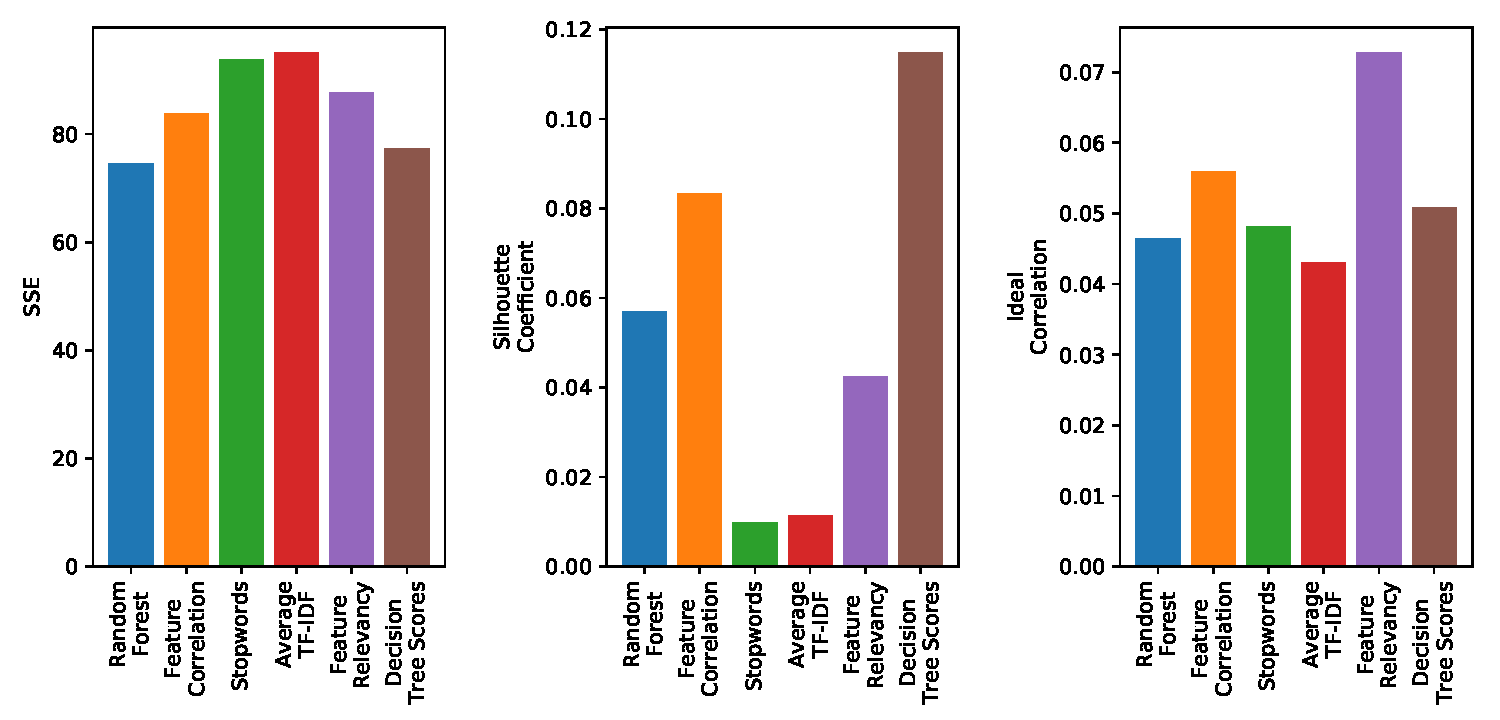
\includegraphics[height=0.3\textheight]{figures/hw3/euclidean/feature_subset_selection}
  \caption{With Euclidean distance as the distance metric for $k$-means clustering, the method for feature subset selection was varied to observe the effects on the resulting clustering's SSE, silhouette coefficient, and ideal-class/cluster similarity matrix correlation.
  Feature-to-class relevancy was found to produce clusters with better purities, but not to the extent that would be useful in accurate classifications.}
\end{figure}

\begin{figure} \label{fig:something}
  \centering
  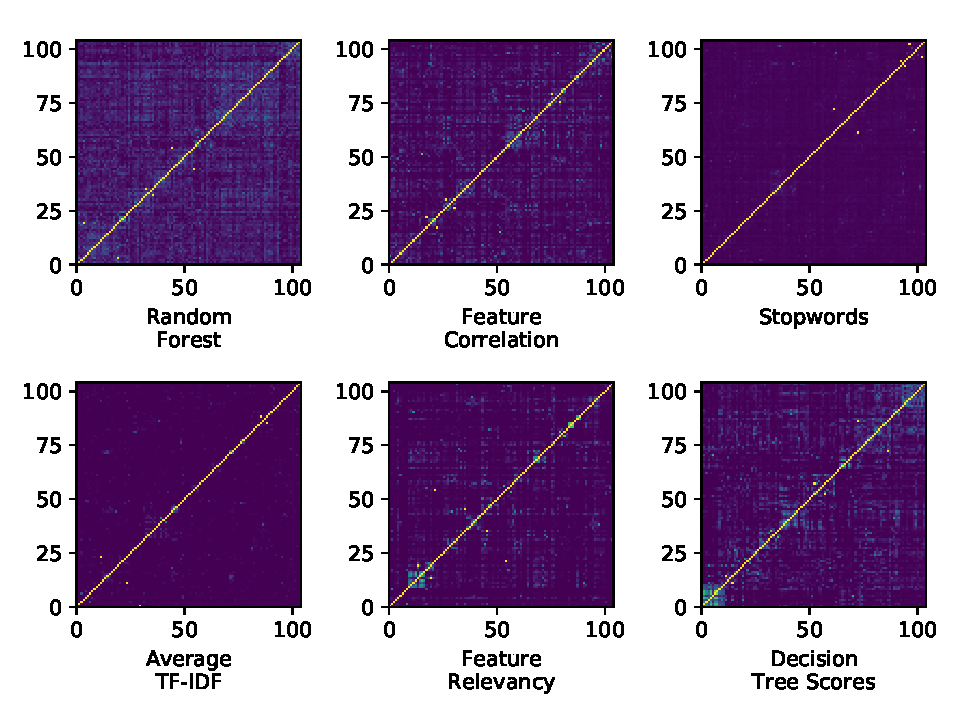
\includegraphics[width=0.8\textwidth]{figures/hw3/euclidean/similarity_matrices}
  \caption{With Euclidean distance as the distance metric for $k$-means clustering, the feature selection methods based on feature-to-class relevancy and decision tree scores permitted $k$-means to produce some clusters with highly similar articles, as is evident in the square structures in the above similarity matrices.}
\end{figure}


\subsection{$k$-means on Cosine Distance} \label{sec:cosine}

With the cosine distance being used in $k$-means, it is again observed in Figure 3 that both the feature selection methods based on average tf-idf scores and the removal of stopwords continue to perform poorly, resulting in clusterings with higher SSEs and lower silhouette coefficients.
However, contrary to its performance under Euclidean distance, the feature relevancy based method drops in its ability to facilitate $k$-means in producing higher quality clusters.
Instead, the decision tree based method for feature selection permits the best clusterings to be produced out of methods tested, resulting in clusters that are more cohesive and better separated (according to its higher silhouette coefficient), as well as closer to the ideal clustering (according to its ideal class/cluster matrix correlation).
This can further be observed in the better-defined structures in its similarity matrix in Figure 4.

It is worth mentioning that the feature correlation method and the random forest method also offer better similarity matrices and more compact clusters, but their effectiveness in producing purer clusters is noticeably less than that of the decision tree method.
However, as was the case in the previous section, the results presented here still suggest that the produced clusters are not suitable for classification.
Even with the decision tree-based feature selection method permitting a clustering that is closest to the ideal, the resulting correlation of approximately 0.067 falls below that of the previous section of approximately 0.07.
Thus, it is inconclusive which distance metrics works better in the $k$-means clustering of the dataset.

%figures/hw3/cosine/feature_subset_selection
%figures/hw3/cosine/natural_clusters
%figures/hw3/cosine/similarity_matrices

\begin{figure}[h!] \label{fig:something}
  \centering
  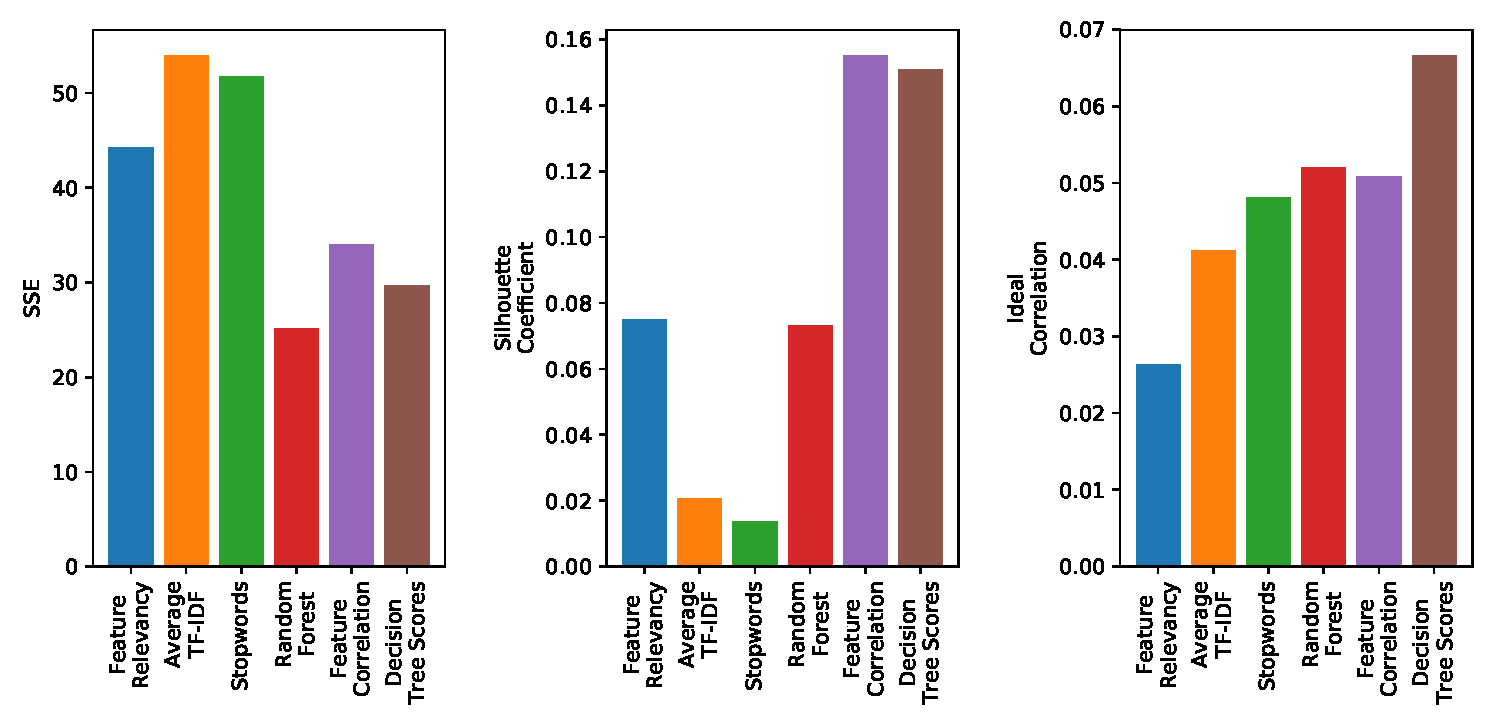
\includegraphics[height=0.27\textheight]{figures/hw3/cosine/feature_subset_selection}
  \caption{With Cosine distance as the distance metric for $k$-means clustering, the method for feature subset selection that permits better clusterings is the decision tree-based method, resulting in clusters that have low SSEs, higher silhouette coefficients, and more correlated to the ideal clustering.}
\end{figure}

\begin{figure}[h!] \label{fig:something}
  \centering
  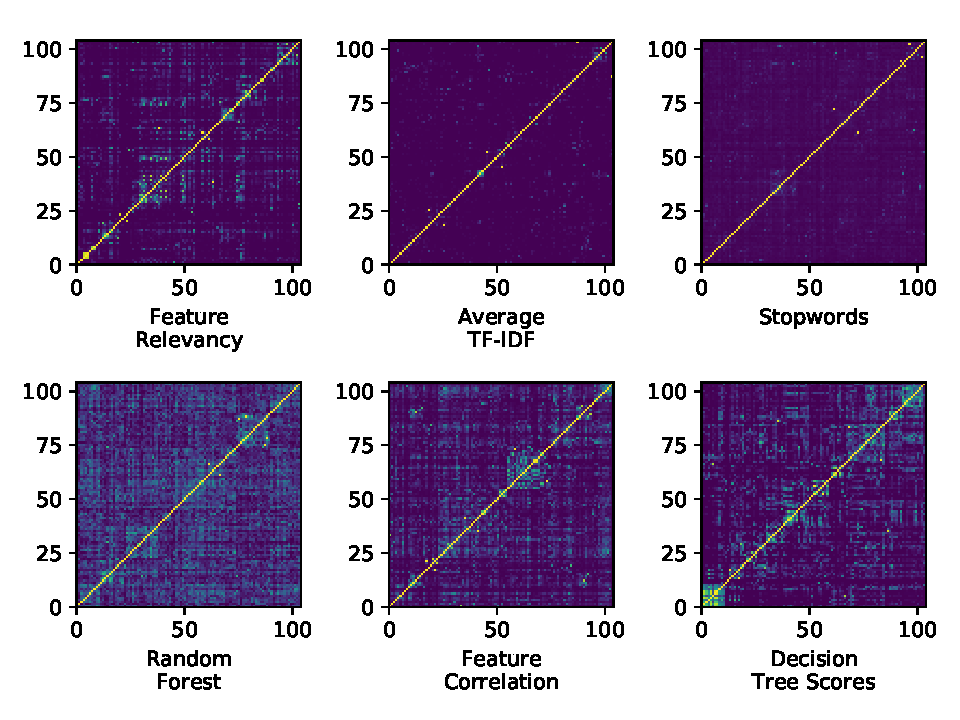
\includegraphics[width=0.8\textwidth]{figures/hw3/cosine/similarity_matrices}
  \caption{With Cosine distance as the distance metric for $k$-means clustering, the clusters resulting from decision tree-based and feature correlation-based feature selection preprocessing appear to consist of articles with higher intra-cluster similarities than inter-cluster.}
\end{figure}


\subsection{$k$-means on the Jaccard Distance} \label{sec:jaccard}

With the Jaccard distance used for $k$-means, the resulting performance is significantly poor across every preprocessing method.
From Figure 5, it is observed that the clusters produced from every feature selection method are nearly equal in terms of their SSEs.
Based on silhouette coefficients, stopword removal and average tf-idf based feature selection methods result in clusters that are very poorly separated and cohesive.
This can be also observed in Figure 6, where there is no discernable pattern in any of the similarity matrices.
Ultimately, this suggests that the Jaccard distance metric is not suitable for $k$-means clustering on a tf-idf representation of articles, as was demonstrated in the previous report.

\begin{figure}[h!] \label{fig:something}
  \centering
  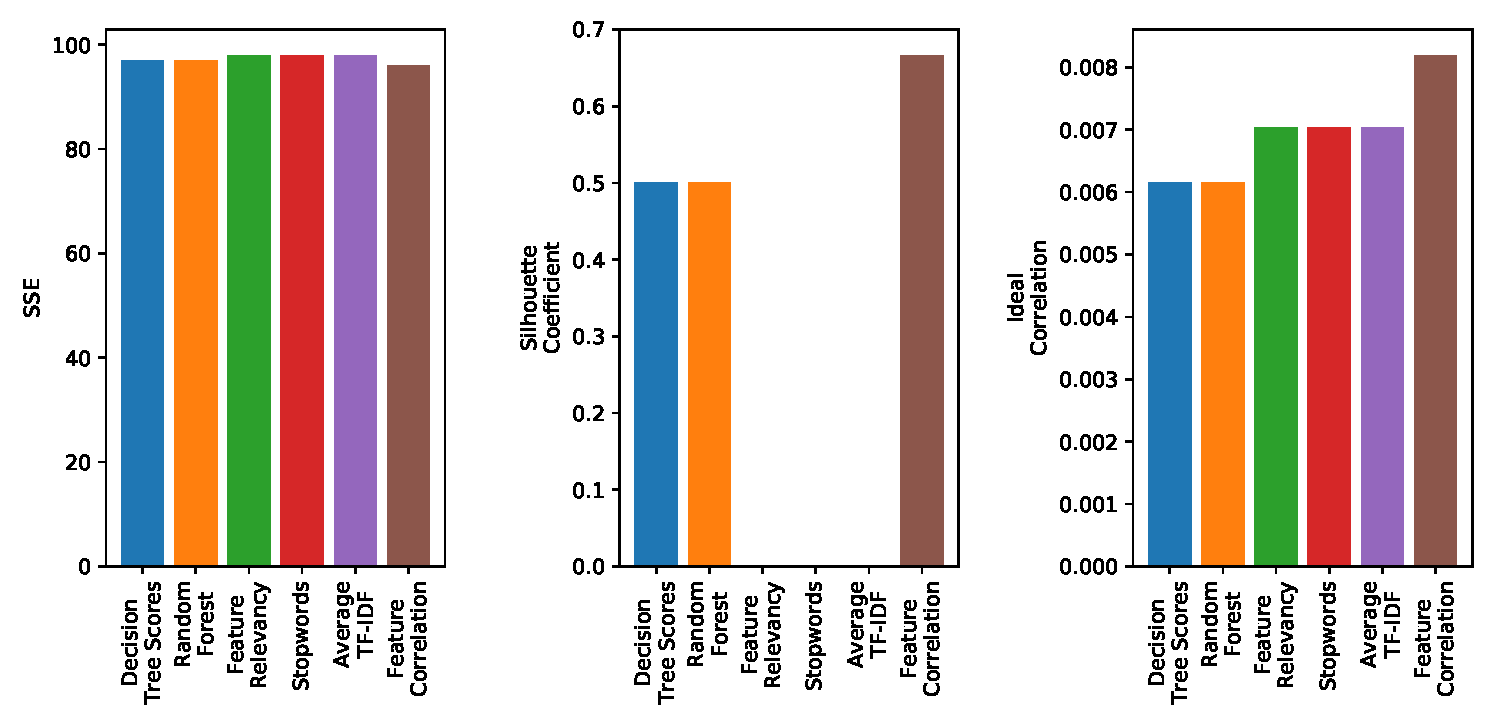
\includegraphics[width=\textwidth]{figures/hw3/jaccard/feature_subset_selection}
  \caption{With the Jaccard distance as the distance metric for $k$-means clustering, no single preprocessing method permitted $k$-means to produce meaningful clusters.}
\end{figure}

\begin{figure}[h!] \label{fig:something}
  \centering
  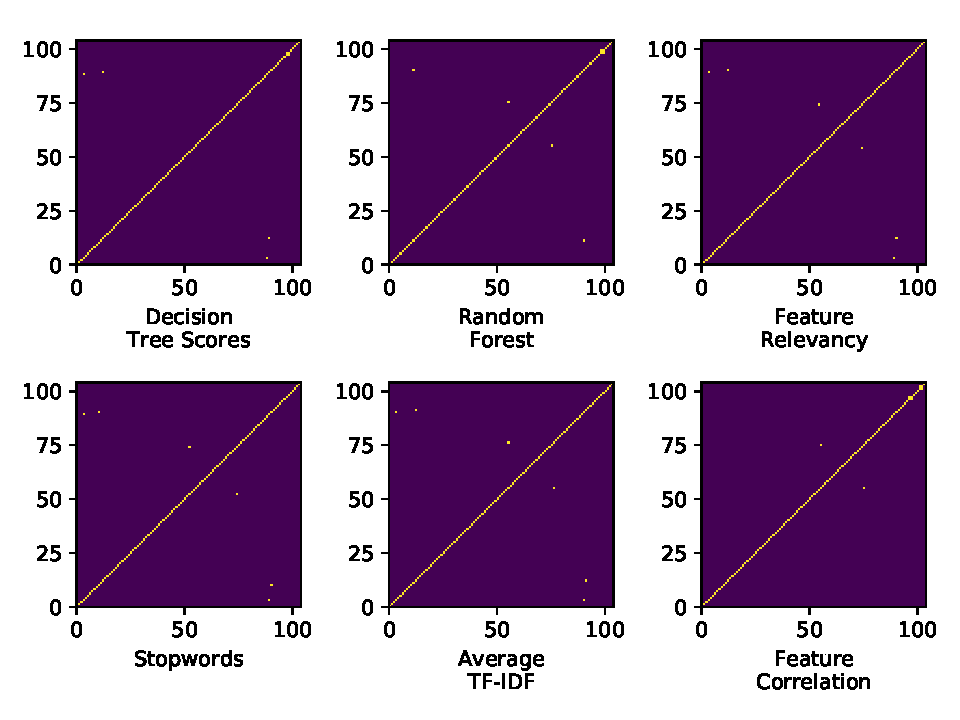
\includegraphics[width=\textwidth]{figures/hw3/jaccard/similarity_matrices}
  \caption{The use of the Jaccard distance as the distance metric for $k$-means clustering resulted in clusters of dissimilar articles.}
\end{figure}


%figures/hw3/jaccard/feature_subset_selection
%figures/hw3/jaccard/natural_clusters
%figures/hw3/jaccard/similarity_matrices

\subsection{Investigating Natural Clusters} \label{sec:natural}

Ideally, the result of a clustering should produce clusters that contain only articles of a particular category.
In the above experiments, the number of clusters constructed by the $k$-means algorithm was equal to the number of article categories.
The results from these experiments indicated that clustering in this manner, under the tested preprocessing methods and distance metrics, could not produce clusters exhibiting a high purity in the classes of articles contained in them.
Because of this, one additional set of experiments was conducted to observe the properties of the clusters produced when the number of clusters to be computed is varied.
For these experiments, the feature-to-class relevancy based method was chosen for feature selection of the dataset during preprocessing, as it was suggested in Section \ref{sec:euclid} to be the best method for facilitating better-quality clusters through $k$-means.
The Euclidean distance and cosine distance are compared to one another, with the Jaccard distance omitted due to its poor performance in Section \ref{sec:jaccard}.

The motivation behind this additional set of experiments is based on the intuition that, although the articles may not be effectively clustered into 7 clusters, there may exist a natural clustering of the articles that results in some class-dominating clusters.
Naturally, this can only occur if the dataset is clustered into 7 or more clusters.
With this intuition, a set of experiments was conducted to observe the overall SSE, silhouette coefficient, and the average purity of the clusters resulting from varying $k$.
The results of these experiences are shown in Figure 7.

From Figure 7, it can be observed that an increase in the number of clusters results in lower SSEs and in increasing silhouette coefficients and average cluster purity.
Because there are more clusters, the SSE of each cluster is expected to decrease due to the centroid-based nature of the $k$-means algorithms.
However, with the silhouette coefficient, there are peaks at $k = 7$ when using the Euclidean distance, and at $k = 9$ and $17$ when using cosine distances.
This suggests that the clusterings produced at those $k$-values are better separated and more cohesive than the clusterings produced by immediately lower and higher $k$ values.
By also observing the average cluster purity, there is a local maxima at $k = 17$ when using both Euclidean distance and cosine distance, suggesting that permitting $k$-means to construct 17 clusters produces clusters of higher purity.
However, they still are not significantly pure so as to be useful in classification.
Due to the small sample size of the dataset, $k$-values higher than 21 produced many singleton clusters, rendering the experimental analysis on those clusterings less meaningful.
Unfortunately, due to time constraints, a more thorough analysis with a larger dataset was not possible for this report.


\begin{figure}[h!] \label{fig:something}
  \centering
  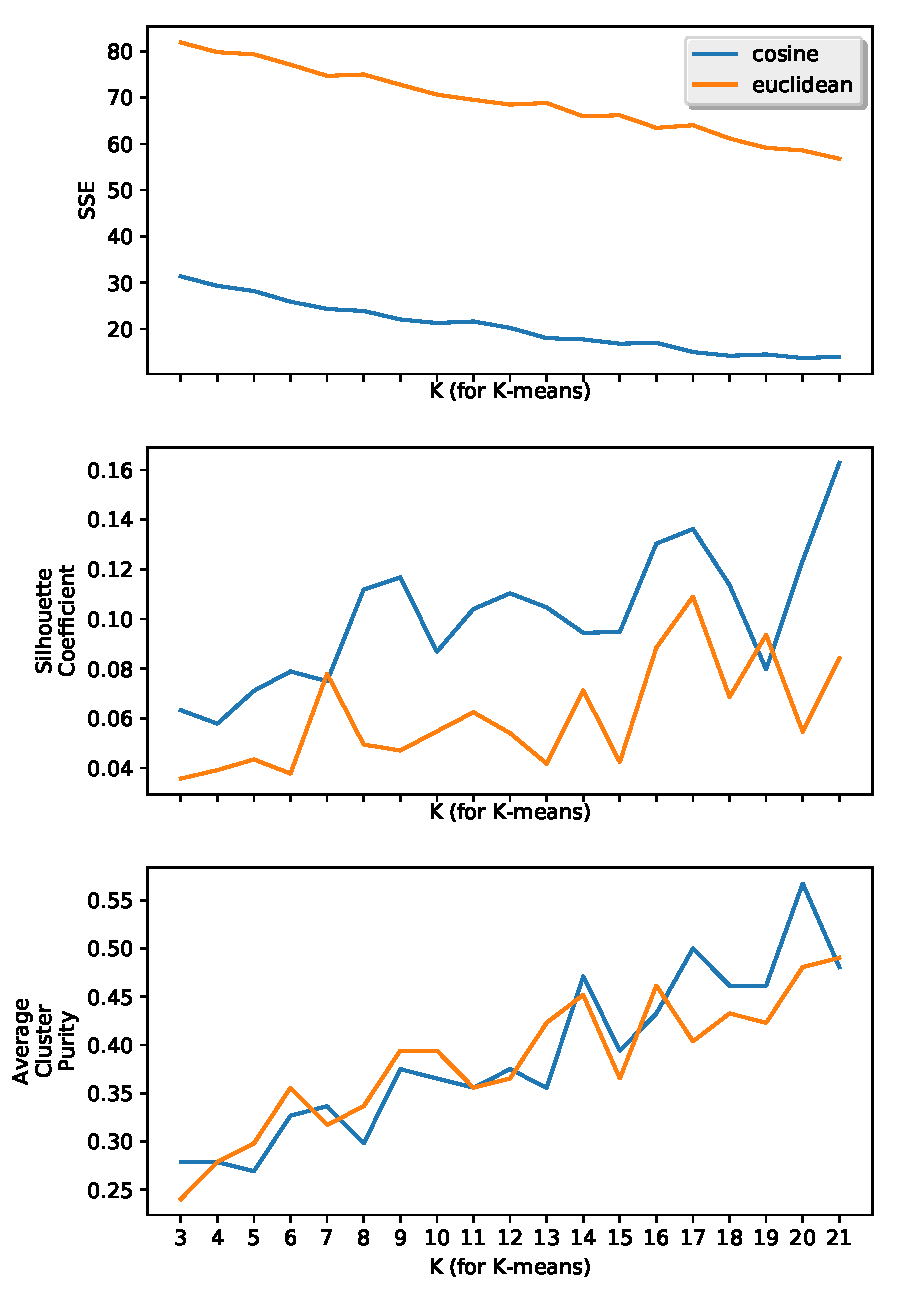
\includegraphics[height=0.6\textheight]{figures/hw3/natural_clusters}
  \caption{When the number of clusters to be found by $k$-means is allowed to increase, the resulting SSE, silhouette coefficients, and average cluster purity is observed to investigate whether there exists a natural clustering of the articles that produces pure category-based clusters.}
\end{figure}

%\begin{figure}[h!] \label{fig:something}
%  \centering
%  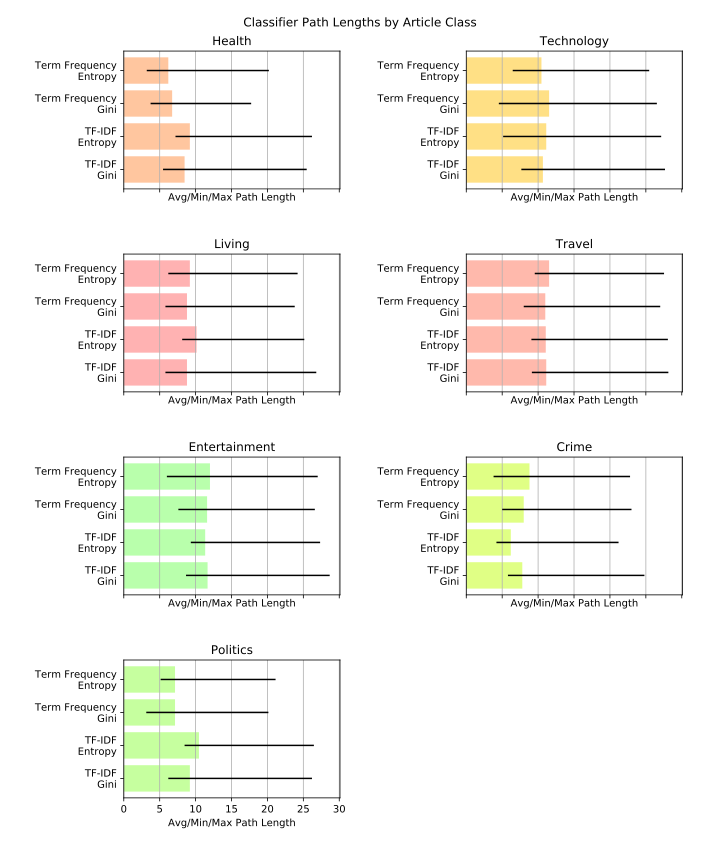
\includegraphics[width=\textwidth]{figures/decision_tree/mrmr/path_depths}
%  \caption{}
%\end{figure}

%\begin{figure}[h!] \label{fig:somethingelse}
%	\centering
%	\begin{subfigure}{.5\textwidth}
%	  \centering
%	  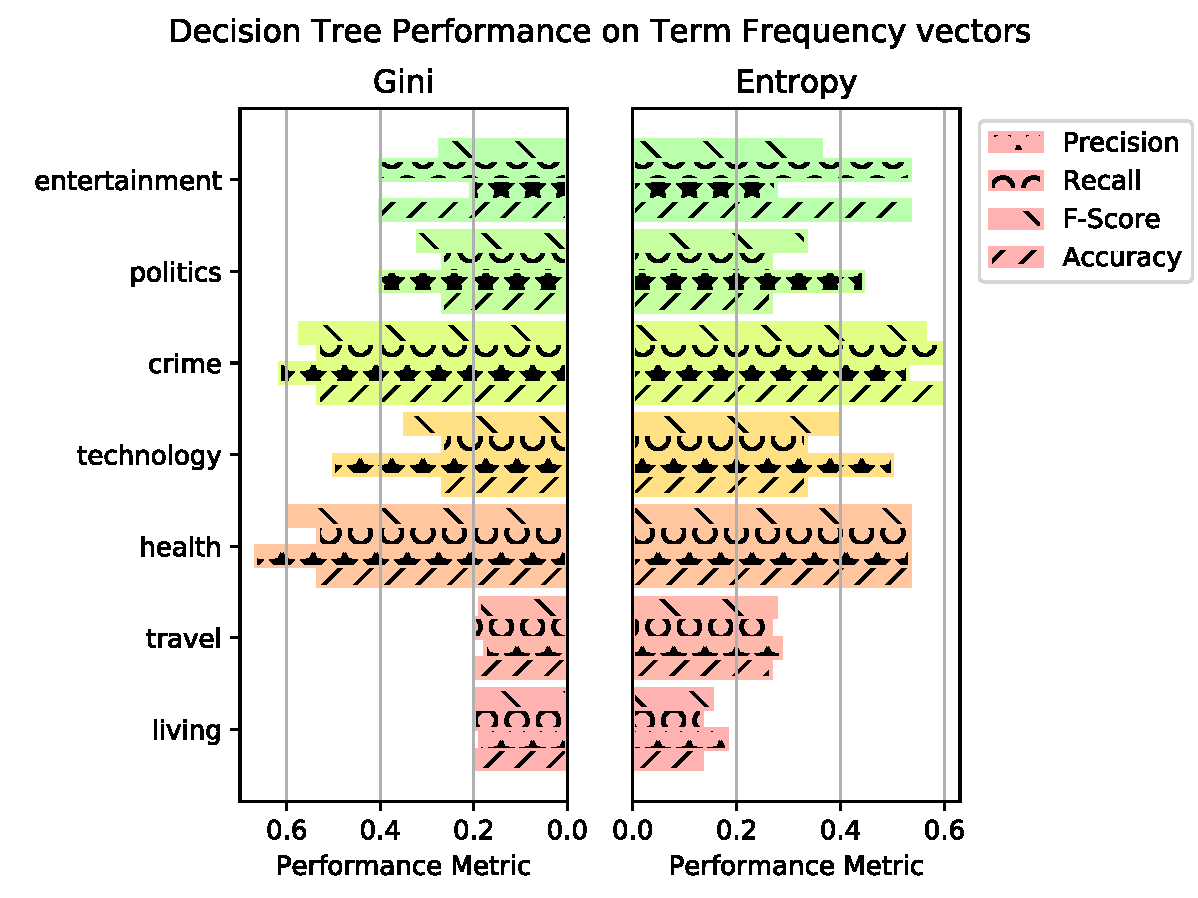
\includegraphics[width=\linewidth]{figures/decision_tree/tf_prec_n_rec}
%	  \caption{}
%	\end{subfigure}%
%	\begin{subfigure}{.5\textwidth}
%	  \centering
%	  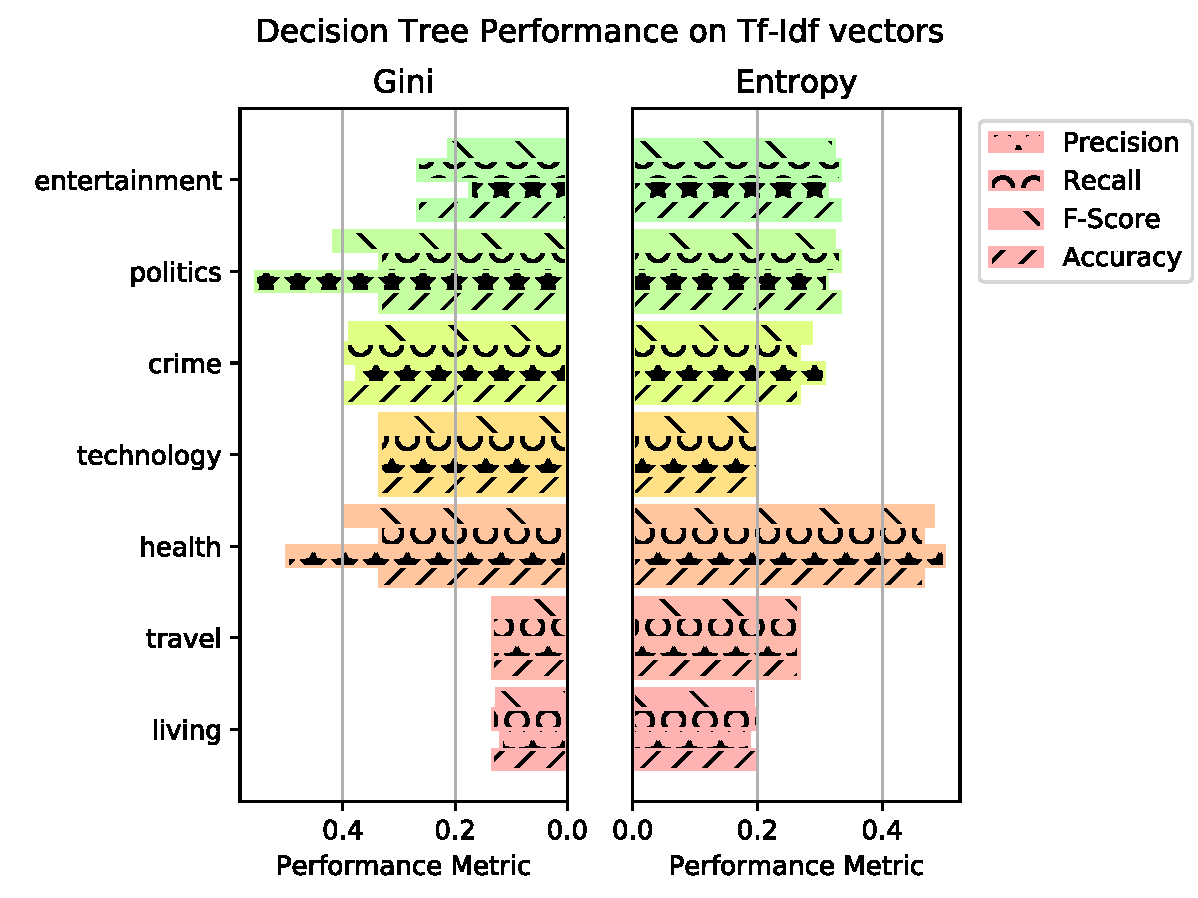
\includegraphics[width=\linewidth]{figures/decision_tree/tfidf_prec_n_rec}
%	  \caption{}
%	\end{subfigure}
%	\caption{}
%\end{figure}


\section{Conclusion} \label{sec:conclusion}

From the above experiments, it is suggested that performing feature selection as a preprocessing step is necessary to improve the results of $k$-means clustering on a dataset of news articles.
Of the tested feature selection methods, the feature-to-class relevancy based method and the decision tree-based method offered better preprocessed datasets when fed into the $k$-means algorithm.
The clusters resulting from these datasets exhibited better compactness and separation, along with higher correlations to the ideal clustering defined by article categories.
However, these clusters were found to be insufficient for performing classification on the articles.
In terms of distance metrics, the Euclidean distance performed slightly better than the cosine distance with regards to the same ideal clustering correlation.
However, the small sample size of the dataset and the very small difference between the results does not permit this finding to be conclusive.
Ultimately, the findings of this report suggest that clustering cannot be used as a single method for classification.
This motivates the investigation of an ensemble approach, in which $k$-means clusterings is but a single factor among many other classification and clustering techniques when one seeks to classify news articles.

\bibliography{bibliography}{}
\bibliographystyle{plain}
\end{document}